\section{Firmware update for embedded devices}
\justify
This chapter details the device firmware update (DFU) mechanisms for BLE-enabled
embedded devices. First of all, the chapter introduces the concepts of DFU.
Subsequently, it provides some examples of existing solutions for DFU based 
on OTA programming. Finally, it presents the system architecture of the prototype
that will be developed as a part of this thesis work. 

\subsection{Device firmware update}
\justify
Device firmware update is the process of updating the software of an operating 
device to a newer version. It aims to deliver fixes and new features to improve 
the system's stability and security. As discussed in Chapter 1, keeping up to date
is becoming more important nowadays, especially for connected devices. 

\justify
In order to perform firmware updates once the device is deployed, the initial
firmware that loaded by the product manufactured has to have the ability to 
load new code without any external programming hardware or tools. Bootloader is 
a mandantory component on every system that supports DFU. Once the microcontroller
resets, bootloader is the first software that is executed. It is responsible for
deciding whether to boot into an existing application or to obtain and install new
firmware image. There are two common approaches when implementing the bootloader:
a single bootloader, and a multi-stage bootloader. Figure 5 shows the memory map 
and the boot flow of a single bootloader. 
\begin{figure}[H]
    \centering
    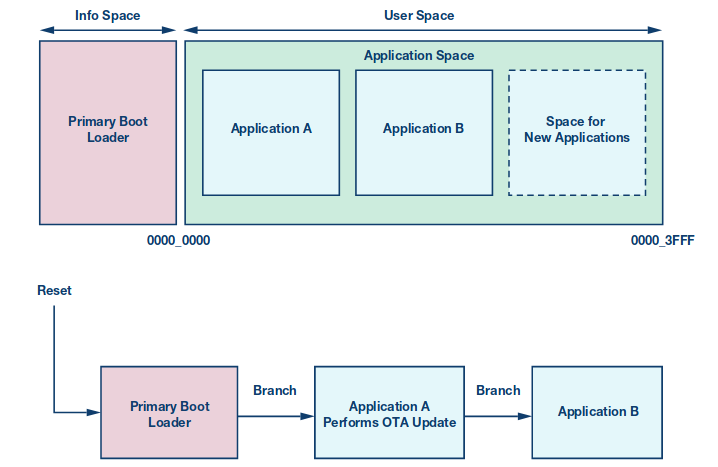
\includegraphics[scale=0.5]{figure/figure05_bl.png}
    \caption{Example memory map and boot flow of a single bootloader.
    Adapted from \cite{ben18}.}
\end{figure}  
\justify
In addition to bootloader, the original application has buit-in functionality for 
the firmware update process. After initiating the update request, either by the 
device itself or by an external party, the original application (for example, 
Application A in figure 5) downloads, verifies and installs the new firmware.
Next, it transfers the control to the new application by performing a branch 
instruction to the reset handler of the new application. However, the drawback 
of this approach is that in some systems, the only safe way to terminate a program 
is through a reset. Another approach is to split the bootloader into separate stages.
Figure 6 demonstrates this implementation in detail.   
\begin{figure}[H]
    \centering
    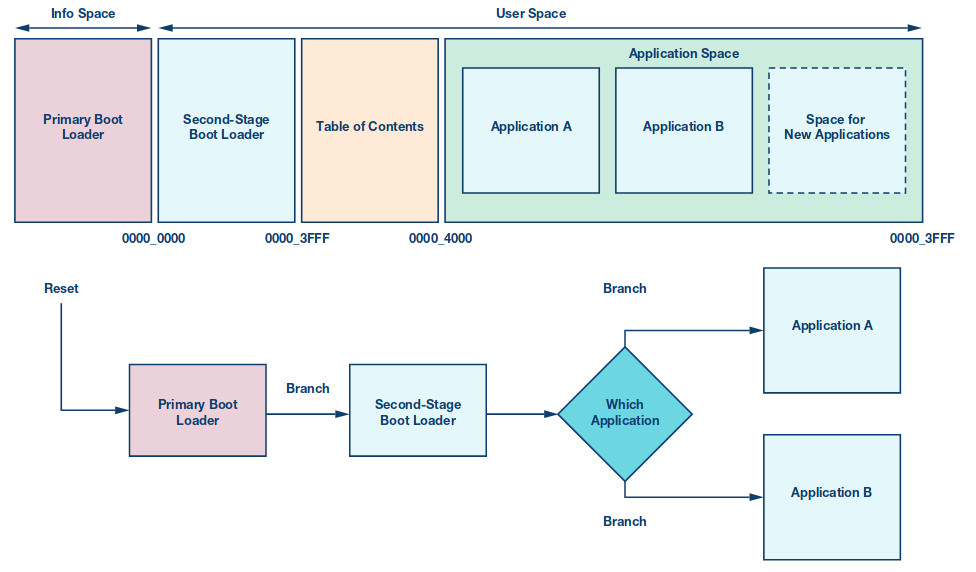
\includegraphics[scale=0.4]{figure/figure06_ssbl.png}
    \caption{Example memory map and boot flow of a multi-stage bootloader.
    Adapted from \cite{ben18}.}
\end{figure}
\justify
The first stage bootloader may offer very limited functionality, such as configuration
of the device, initialisation of primary peripherals, and preparation for next stage
bootloaders. Some hardware vendor hardcodes this type of bootloader in the device,
thus cannot be changed by users. The second stage bootloader may implement more
complex functionality. It can either initiate the firmware update process, or boot 
into the desired application. With this approach, the application can get rid of large
amount of update-related code. To perform an update while the device is operating,
a pre-defined value indicating update request is set to one special register, which 
do not change after rebooting the device, followed by a soft reset triggered by the
application. After the second stage bootloader has been loaded, it acknowledges the 
request and branches into firmware update process. As a result, multi-stage
bootloader reduces the code duplication and simplifies the application specific 
software. 

\justify
Another important consideration when designing a firmware update process is the 
choice of data transportation protocol. Common communication protocols, such as 
UART, USB, SPI, BLE, LoRaWAN, and so on, can be leveraged to transmit the new 
firmware from a master device to other slave devices. The decision on which protocol 
to use depending on how the update process carries out. For in-field firmware update, 
it is usually performed by a human and requires a physical connection between the 
microcontroller and the updater tool. The advantage of this method is that in case
of update error, the operator can manually retry the process. For over-the-air 
firmware update, a wireless connectivity is required to manage the update process.
The running application manages its own firmware update through the mechanism 
described above. This method can scale to a large number of devices and require 
minimal human effort. However in case of update error, retry may be difficult
to support.

\justify
There are many challenges that the designers have to address when developing 
the firmware update mechanism. First, the developers have to choose a suitable
binary format for the application and the method of delivering and organising
data in the target system. Since most of the application binary is too large 
to fit in single transfer, the data are often be splitted and delivered in chunks.
Depending on the system constrains, the bootloader should implement an efficient 
strategy to verify the incomming data and commit them to the flash. Next, the
update process can fail for various reasons such as transmission error, 
transmission failure, transmission loss, or the new firmware does not function
properly. Hence the system should be able to detect theses issues and take 
appropriate actions to preserve the availability and responsiveness. Finally,
the design of the system must address common security threats. The bootloader 
must be able to verify that the new firmware is from a trusted party. The data
sending from the master device must also be encrypted and not corrupted when 
arriving at the slave device. 

% \justify
% It is obviously a quite challenging task to develop a firmware update process for
% embedded devices. Depending on the application, several factors must be taken into
% account during the planning phase. Once the design has been done right, the devices 
% are likely to operate properly and safely during their lifetime with the most 
% up-to-date firmware.

\subsection{Over-the-air (OTA) programming}
\justify
Over-the-air programming is a mechanism to deliver the firmware update wirelessly, 
without requiring physical access to the device. Depending on the requirements 
of the application, there are several choices of wireless communication protocols. 
For example, if the device is a smartwatch, the users' phone can transfer the data 
through short-range radios such as BLE. In contrast, a wireless sensor network 
scattering a city may require long-range radios such as LoRaWAN or cellular 
networks. 

% Characteristics and benefits of OTA

%   Over-the-air firmware updates:
%       stand alone update operation
%       uses device connectivity to receive and manage the update
%       running application manages its own firmware update
%       retry may be difficult to support

% Limitation and chalenges of OTA
%   Same as described above
%   Due to limitation of payload, the new firmware has to be packetized
%       challenges in organizing the incoming data
%   The hardware and software must be designed with OTA update in mind
%   from the beginning of the project

